\begin{frame}
\frametitle{Breathing to regulate tension}
%\begin{columns}[c] % The "c" option specifies centered vertical alignment while the "t" option is used for top vertical alignment

%\column{.7\textwidth} % Left column and width
%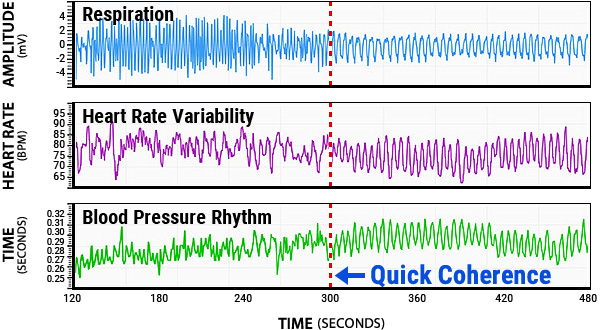
\includegraphics[width=\linewidth]{graph-coherence.jpg}
%\column{.3\textwidth} % Right column and width
 
%\end{columns}

You can \structure{optimise tensions} in your body already with the means of the \structure{breath} alone. 

Are you one of the calmer people, who could profit from a bit more of tension? Or do you belong to the more active or over active people, who have a hard time getting rid of their tension?

Choose your exercise!

\end{frame}

%-----------------------------------------------------------------------------------------------------------------

\begin{frame}
\frametitle{Build up/release tension}
%\begin{columns}[c] % The "c" option specifies centered vertical alignment while the "t" option is used for top vertical alignment

%\column{.7\textwidth} % Left column and width
%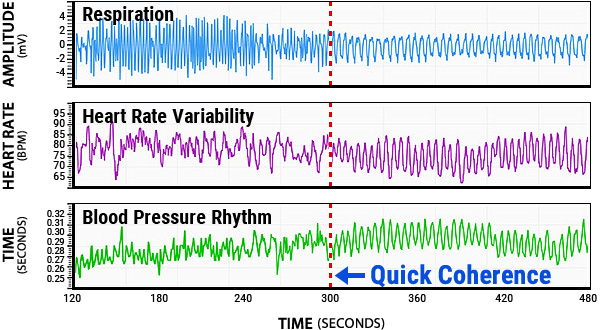
\includegraphics[width=\linewidth]{graph-coherence.jpg}
%\column{.3\textwidth} % Right column and width
 
%\end{columns}
\begin{itemize}
\item[1. ] \textbf{\structure{Builds up tension}, for example while being tired:}

Hold your \structure{left nose hole closed} and \structure{inhale} trough the right one. To exhale you \structure{close your right nose hole} and \structure{exhale through the left one}.
\item [2. ] \textbf{\structure{Releases tension}:}

Hold your \structure{right nose hole closed} and \structure{inhale} trough the left one. To exhale you \structure{close your left nose hole} and \structure{exhale through the right one}.
\end{itemize}
\end{frame}

%-----------------------------------------------------------------------------------------------------------------

\begin{frame}
\frametitle{ tension}
%\begin{columns}[c] % The "c" option specifies centered vertical alignment while the "t" option is used for top vertical alignment

%\column{.7\textwidth} % Left column and width
%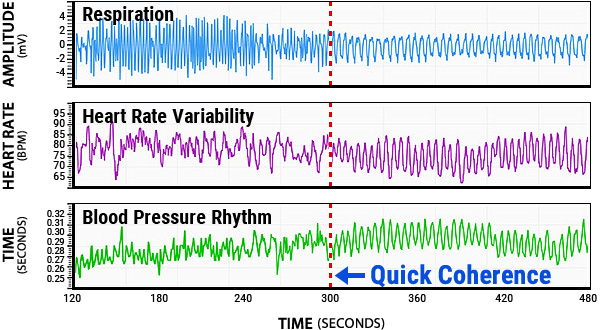
\includegraphics[width=\linewidth]{graph-coherence.jpg}
%\column{.3\textwidth} % Right column and width
 
%\end{columns}
\begin{itemize}
\item[3. ] \textbf{\structure{Builds up tension}, for example while being tired:}

Hold your \structure{left nose hole closed} and \structure{inhale} trough the right one. To exhale you \structure{close your right nose hole} and \structure{exhale through the left one}.

Hold your \structure{right nose hole closed} and \structure{inhale} trough the left one. To exhale you \structure{close your left nose hole} and \structure{exhale through the right one}.
\end{itemize}
\end{frame}